\documentclass[a4paper]{article}

\usepackage{linus-style}
\setdefaultlanguage{french}

\usepackage[colorlinks=true,urlcolor=blue]{hyperref}
\usepackage{graphicx}

\title{Dessin de plantes}
\author{Cristian Trout et Linus Heckemann}
\date{février -- mai 2014}

\begin{document}
\maketitle

\section{Le sujet choisi}
C’est un constat que beaucoup de plantes ont des physionomies qui rappellent des fractales, c’est-à-dire ont des formes qui se répètent en agrandissant ou rapetissant. Voici par exemple, le chou-fleur Romanesco.

\hspace{\fill}\includegraphics[width=0.4\textwidth]{rapport/Fractal_Broccoli}\hspace{\fill}

Vu la facilité des ordinateurs d’exécuter des actions répétitives et vu la pénibilité pour nous de dessiner quelque chose répétitivement et méticuleusement, il serait intéressant de coder un programme qui peut dessiner ces plantes à notre place. Notre problème est donc le suivant: 
Comment créer un programme qui peut construire une structure de fractale mais qui permettrait aussi d’incorporer des touches naturelles et aléatoires à la structure en question? Et puis comment traduire cette structure en quelque chose représenté?

\section{Le but visé et les moyens choisis}
Après des recherches, nous avons décidé d’utiliser une système de Lindenmayer (L-Système) comme méthode pour construire nos structures: elle permet de créer des structures récursives, comme les fractales et offre beaucoup de flexibilité et de contrôle.

\section{Détail de l'algorithme}
Un L-Système consiste d’un <<~alphabet~>> de symboles qui sont soit variables soit  constants, de <<~règles~>> de reproduction (qui associe à chaque symbole un ou plusieurs autre(s) symbole(s) et un axiome. Un L-système est un processus qui crée une liste structurée de ses symboles. Voici le déroulé du processus:

On lit la liste initiale, génération n (l’axiome dans le cas de la génération 0)
D’après les règles établies, on remplace dans la liste tous les symboles variables avec leurs symboles correspondant
On ne change pas les constantes
Sortie de la liste de génération n+1

Ce processus est répété autant de fois voulu et (généralement) la liste devient plus complexe avec chaque nouvelle génération de la liste.  \href{http://fr.wikipedia.org/wiki/L-système}{L'article Wikipedia} sur le sujet présente d'autres exemples de ce que l'on peut modéliser avec les L-systèmes.

La structure fondamentale du code se base autour d’un L-Système:

Les générations et l'état final du système est encodé par une variable de type list car les listes sont très flexibles et chaque symbole dans la liste est un type string (pour pouvoir leur donner des noms explicites).
Les règles sont encodés par une variable de type dict car un dictionnaire est fait pour associer des variables avec d’autres variables
Une boucle for fait répéter le processus autant de fois voulu

Apres avoir évalué le nombre de générations voulu, on fait lire la liste et à chaque symbole on associe une fonction qui contribuera à la création de l’image final. L’exécution de ces fonctions dans l’ordre donné par la liste débouche sur une image avec des motifs récursifs, dans nos  deux cas, celle d’une fougère et celle d'un arbre.

Pour ajouter des touches aléatoires on associe, tout simplement, des probabilités soit aux règles du L-Système (un symbole donnera des chaînes de symboles variables, comme dans l'exemple de l'arbre. On l’appelle alors un L-Système stochastique) soit aux actions auxquels les symboles correspondent, soit les deux.

\section{Collaboration au cours du projet, le travail en équipe}
Au début, Cristian a implémenté lui-même un programme qui dessinait une fougère en se servant du turtle seulement. Nous avons ensuite intégré cela dans une structure élaborée par Linus qui permet la généralisation et l'encapsulation des parties différentes (évaluation du système, rendu\dots). Grâce à cela, nous pouvons facilement changer de système de rendu -- voir par exemple la fonction \verb main  dans \verb fern.py . Nous pouvons ainsi aussi générer les structures dans Blender, ce qui, avec quelques modifications du code, nous permettrait de faire des plantes tridimensionnelles.

Nous avons travaillé ensemble en nous servant d'un logiciel de \href{http://fr.wikipedia.org/wiki/Gestion_de_versions}{gestion de versions} appelé \href{http://git-scm.org/}{git}, qui nous a permis de travailler sur le code en même temps et de consolider notre travail. Nous nous sommes servis de Skype\texttrademark{} pour communiquer, mais à cause de problèmes de contact nous n'avons pas travaillé de la manière la plus efficace.

\hspace{\fill}\includegraphics[width=0.5\textwidth]{rapport/git-history}\hspace{\fill}

\hspace{\fill}\emph{L'histoire de notre projet (Bobbster = Cristian)}\hspace{\fill}



\section{Les difficultés rencontrées}
Nos difficultés ont été pour la plupart en rapport avec la faible communication au cours de la réalisation du projet, qui a résulté dans une mauvaise gestion du temps.

À part cela, l'évaluation contextuelle des L-systèmes, qui a été très utile pour le dessin de l'arbre, a nécessité une réorganisation de la structure interne de l'évaluation des L-systèmes (dans la classe \verb lsys.core.System ) et une séparation plus forte entre l'évaluation du système et le rendu du résultat. L'évaluation et le rendu du système sont maintenant complètement séparés l'un de l'autre, et les deux étapes sont consolidées dans une autre classe.

La troisième et la dernière difficulté que nous avons rencontrée est celle de la performance.

\hspace{\fill}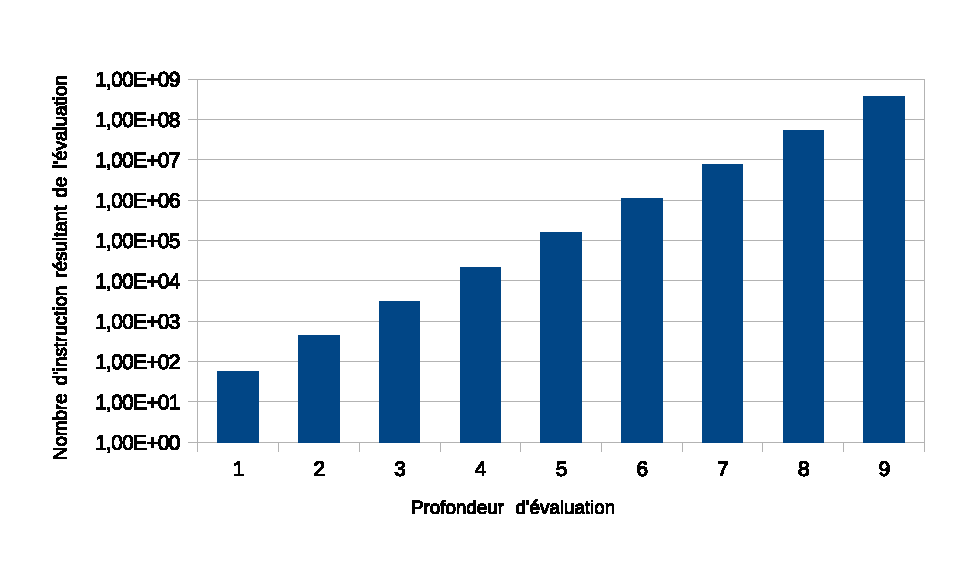
\includegraphics[width=0.8\textwidth]{rapport/instructions}\hspace{\fill}

{\centering\emph{Nombre d'instructions de rendu générées en fonction de la profondeur d'évaluation, pour l'exemple de la fougère}}

On voit une augmentation à peu près exponentielle du nombre d'instructions quand la profondeur augmente. C'est pour cela qu'il est difficile de faire un rendu à une grande profondeur, même si on optimise beaucoup: il faut améliorer la performance d'un facteur d'environ 8 pour avoir la même vitesse de rendu à une profondeur augmentée de 1. 

\section{Éventuelles améliorations}
Le processus du L-système étant très général, il pourrait être appliqué dans de très nombreux domaines, qui ne se limitent pas au graphique. Nous avons par exemple eu l'idée d'essayer de générer de la musique en nous en servant; notre recherche sur ce point n'est pas encore aboutie.

Une amélioration de facteur 8 ou même plus de la performance serait peut-être possible en réécrivant le code du rendu en C et en l'appliquant comme module d'extension qui sera ensuite importé et pourra donner une quatrième option pour le rendu. Pourtant, Blender est déjà très efficace pour l'affichage donc ce ne serait probablement qu'une amélioration par rapport au systèmes de rendu actuels qui s'appuient sur turtle et sur OpenGL mais en python.

Comme déjà mentionné, une autre amélioration à faire serait d'implémenter la 3D.

\end{document}